\begin{center}
	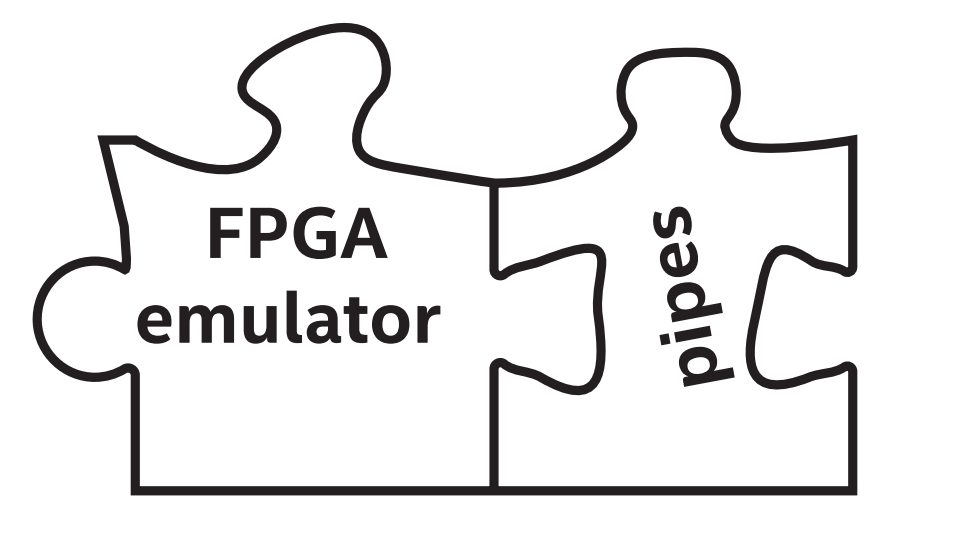
\includegraphics[width=0.5\textwidth]{content/chapter-17/images/1}
\end{center}

Kernel-based programming originally became popular as a way to access GPUs. Since it has now been generalized across many types of accelerators, it is important to understand how our style of programming affects the mapping of code to an FPGA as well.\par

Field Programmable Gate Arrays (FPGAs) are unfamiliar to the majority of software developers, in part because most desktop computers don’t include an FPGA alongside the typical CPU and GPU. But FPGAs are worth knowing about because they offer advantages in many applications. The same questions need to be asked as we would of other accelerators, such as “When should I use an FPGA?”, “What parts of my applications should be offloaded to FPGA?”, and “How do I write code that performs well on an FPGA?”\par

This chapter gives us the knowledge to start answering those questions, at least to the point where we can decide whether an FPGA is interesting for our applications, and to know which constructs are commonly used to achieve performance. This chapter is the launching point from which we can then read vendor documentation to fill in details for specific products and toolchains. We begin with an overview of how programs can map to spatial architectures such as FPGAs, followed by discussion of some properties that make FPGAs a good choice as an accelerator, and we finish by introducing the programming constructs used to achieve performance.

The “How to Think About FPGAs” section in this chapter is applicable to thinking about any FPGA. SYCL allows vendors to specify devices beyond CPUs and GPUs, but does not specifically say how to support an FPGA. The specific vendor support for FPGAs is currently unique to DPC++, namely, FPGA selectors and pipes. FPGA selectors and pipes are the only DPC++ extensions used in this chapter. It is hoped that vendors will converge on similar or compatible means of supporting FPGAs, and this is encouraged by DPC++ as an open source project.\par






















































